\documentclass[RNAAS]{aastex631}

% Numbers are \input from the pipeline-generated macros -- none typed by hand.
% Auto-generated by jansky_research.vgpra._write_macros -- do not edit.
% vgSyn* = synthetic recover-a-known (always live); vgReal{U,N}* = real Uranus/Neptune legs.
\newcommand{\vgSource}{PDS-PPI Voyager 2 PRA low-band 6-s encounter volumes (Uranus + Neptune)}
\newcommand{\vgSynInjected}{17.24}
\newcommand{\vgSynRecovered}{17.22252}
\newcommand{\vgSynSigma}{0.02049}
\newcommand{\vgSynRayPeriod}{17.24308}
\newcommand{\vgSynRecoveredOK}{yes}
\newcommand{\vgSynRayOK}{yes}
\newcommand{\vgRealUPeriod}{18.44362}
\newcommand{\vgRealUSigma}{1.94272}
\newcommand{\vgRealULo}{14.41862}
\newcommand{\vgRealUHi}{18.67411}
\newcommand{\vgRealURayPeriod}{14.72424}
\newcommand{\vgRealUSpan}{312.0}
\newcommand{\vgRealUUnc}{1.94272}
\newcommand{\vgRealUSpread}{1.75737}
\newcommand{\vgRealURecovers}{no}
\newcommand{\vgRealUHist}{17.24}
\newcommand{\vgRealUHistOK}{yes}
\newcommand{\vgRealNPeriod}{20.0}
\newcommand{\vgRealNSigma}{1.94042}
\newcommand{\vgRealNLo}{15.84267}
\newcommand{\vgRealNHi}{20.0}
\newcommand{\vgRealNRayPeriod}{15.95265}
\newcommand{\vgRealNSpan}{504.0}
\newcommand{\vgRealNUnc}{1.94042}
\newcommand{\vgRealNSpread}{0.70181}
\newcommand{\vgRealNRecovers}{no}
\newcommand{\vgRealNHist}{16.11}
\newcommand{\vgRealNHistOK}{no}
\newcommand{\vgRealULamy}{17.247864}
\newcommand{\vgRealULamyOK}{yes}


\newcommand{\code}[1]{\texttt{#1}}

\begin{document}

\title{A Blind Reanalysis of the Voyager~2 PRA Data Recovers Neither the Uranus nor the
Neptune Rotation Period}

\author[0009-0008-3289-4447]{Joseph Barbere}
\affiliation{Independent researcher}

\begin{abstract}
The radio rotation periods anchoring the System~III longitudes of Uranus
(\vgRealUHist~h) and Neptune (\vgRealNHist~h) were fixed by the Voyager~2 Planetary
Radio Astronomy (PRA) experiment during the 1986 and 1989 flybys
\citep{warwick1986,warwick1989} and, for the radio data, revisited only once
(\citealt{lecacheux1993} refined Neptune's to $16.108\pm0.006$~h from the same flyby);
neither period has been reanalysed with a blind, un-modelled periodogram or modern
statistics, even as \citet{lamy2025} recently refined Uranus to \vgRealULamy~h from
Hubble UV aurorae. Using a small,
tested tool (\code{vgpra}), I ask what a blind Lomb--Scargle periodogram of the open
PDS-PPI PRA flux \citep{pdsppi_vg2pra} recovers over an un-tuned 14--20~h window, using
none of the historical emission-beaming or magnetic-longitude modelling. The answer is
a controlled null: the pipeline recovers an injected synthetic rotation
(\vgSynInjected~h $\to$ \vgSynRecovered~h) to $\sim$1~min but recovers neither real
period, and injections into the real series bound any rotational modulation at the
historical periods to depths below \vgRealUMinDepth\% (Uranus) and \vgRealNMinDepth\% (Neptune). This is a reproducibility-and-limits note, not a new measurement.
\end{abstract}

\section{Result}

\code{vgpra} \citep{janskyresearch} builds a band-integrated total-power flux series from the
open PDS-PPI Voyager~2 PRA low-band 6-second encounter volumes \citep{pdsppi_vg2pra}
and searches it with a blind Lomb--Scargle periodogram over a wide, deliberately
un-tuned 14--20~h ice-giant window, not centred on the known answers, since a
narrow window would manufacture a match. A historical period counts as \emph{recovered}
only if the blind peak lands within one combined-$\sigma$ of it (rotation-block bootstrap
plus sub-band spread), is band-robust (spread $<0.6$~h across three disjoint thirds of the
100--1000~kHz analysis band), and is not railed to a search bound. The window and criterion
changed twice after real results were seen, and both changes are disclosed: an earlier,
narrower window reported Neptune as recovered near 16~h, so the window was widened and the
band-robustness and railing clauses added; and an earlier sub-band set included one band
above the analysis band, which alone decided the Uranus verdict, so the bands were
redefined as disjoint thirds. The scramble and injection controls below are likewise post
hoc. The final rule was applied identically to both planets and to a synthetic control, which recovers its injected period
(\vgSynInjected~h $\to$ \vgSynRecovered~h) and passes the full rule (\vgSynFullOK).

On the real encounter volumes the blind periodogram recovers neither planet
(Figure~\ref{fig:vgpra}). The Uranus peak sits at \vgRealUPeriod~h, 1.1 resolution
elements (\vgRealURes~h) above the historical \vgRealUHist~h, and its sub-band peaks have a standard deviation of
\vgRealUSpread~h, one of them railed, so it is not a stable line and is not recovered. It
is inconsistent with white noise (scramble FAP $\le\vgRealUFap$ over \vgRealUNIndep\
independent frequencies), but a scramble also destroys red noise and the flyby envelope,
so this shows structure in the series, not a coherent line. The bootstrap width is nearly that of the search window, so it reports
an unconstrained peak rather than an uncertainty, and the historical and Hubble values
lying within it says nothing. The Neptune peak rails to the upper search bound
(\vgRealNPeriod~h); a railed peak is a bound, not an estimate, so no consistency statement
with \vgRealNHist~h is possible, and it is not recovered.

The operative validation is an injection into the real series (red noise, flyby envelope
and detrend included): a fractional sinusoid at each historical period is recovered in
every one of eight phases at modulation depths of \vgRealUMinDepth\% (Uranus) and
\vgRealNMinDepth\% (Neptune), the smallest tested depths to reach that, on a grid stepping by
factors of two. A sinusoidal total-power modulation at the historical period is therefore
excluded at those depths; the bound lies between half and all of each value. The auroral total-power flux is therefore not a clean
rotational sinusoid over these flybys, consistent with the beaming and magnetic-longitude
modelling of the original determinations, which a blind periodogram omits, having been
necessary; this analysis does not test that modelling. Every measured value above is
\code{\textbackslash input} from a pipeline-generated macro file and regenerates from a
clean checkout (\code{python -m jansky\_research.vgpra}).

\begin{figure}[h!]
\centering
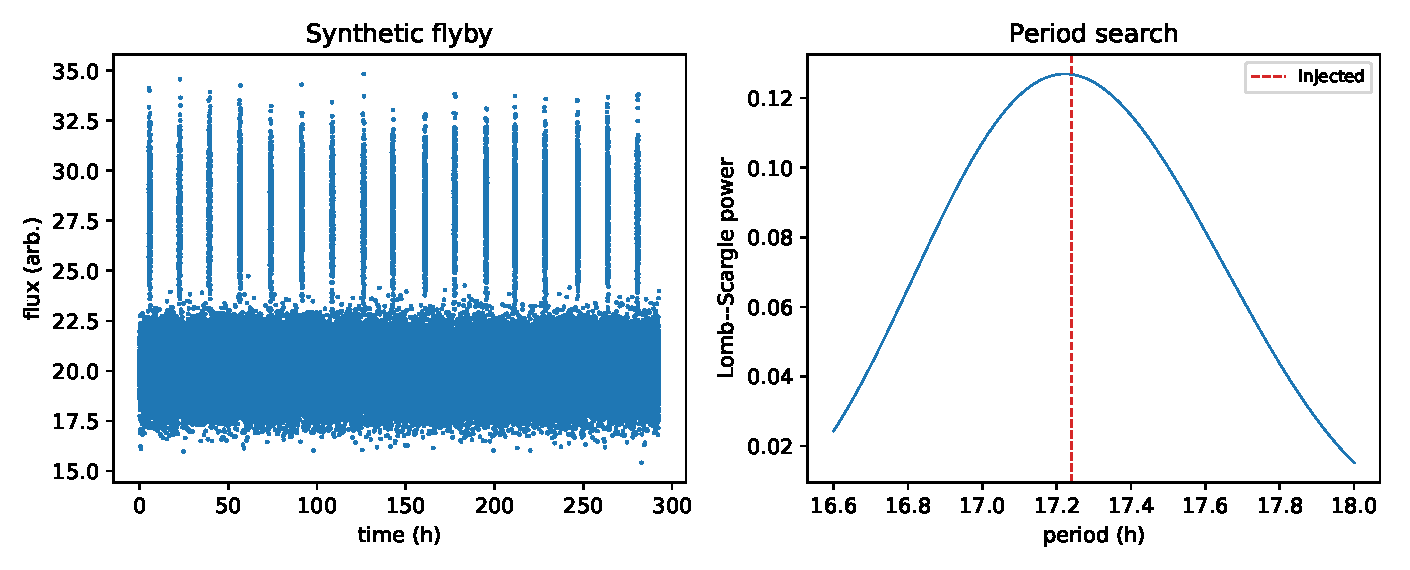
\includegraphics[width=0.7\linewidth]{figures/vgpra.pdf}
\caption{Blind Lomb--Scargle reanalysis of the Voyager~2 PRA flux, computed by
\code{vgpra}, over the full un-tuned 14--20~h window: the synthetic control (left;
injected \vgSynInjected~h, recovered \vgSynRecovered~h) and the real Uranus and Neptune
series (middle, right; historical periods dashed, blind peaks dotted). Neither real peak coincides with its historical period; Neptune's rails to the window bound.}
\label{fig:vgpra}
\end{figure}

\begin{acknowledgments}
Developed collaboratively with Anthropic's Claude \citep{anthropicclaude} (a large
language model); the author directed and verified the work, and an AI assistant is not
an eligible author. Thanks to the NASA PDS Planetary Plasma Interactions node for the
open Voyager~2 PRA archive.
\end{acknowledgments}

\software{jansky-research \citep{janskyresearch}, Astropy \citep{astropy2022}, NumPy,
SciPy, jansky \citep{jansky}}

\bibliographystyle{aasjournal}
\bibliography{refs}

\end{document}
